% =====================================================================
%  LIAR Truth Detector - project report
%  Compile on Overleaf (pdfLaTeX). Upload this folder (main.tex + figures/).
% =====================================================================
\documentclass[11pt,a4paper]{article}

% ---------- page and fonts ----------
\usepackage[T1]{fontenc}
\usepackage[utf8]{inputenc}
\usepackage{mathpazo}                 % Palatino-style body text
\usepackage[scaled=0.92]{helvet}      % Sans-serif for headings and captions
\usepackage{microtype}
\usepackage[a4paper,margin=2.4cm]{geometry}
\usepackage{setspace}
\setstretch{1.12}
\usepackage{parskip}
\setlength{\parskip}{0.55em}

% ---------- colours (same palette as the figures) ----------
\usepackage[table]{xcolor}
\definecolor{brandblue}{HTML}{2A78D6}
\definecolor{brandorange}{HTML}{EB6834}
\definecolor{brandaqua}{HTML}{1BAF7A}
\definecolor{ink}{HTML}{0B0B0B}
\definecolor{softgray}{HTML}{F3F2EF}
\definecolor{midgray}{HTML}{52514E}

% ---------- graphics, tables, boxes ----------
\usepackage{graphicx}
\graphicspath{{figures/}}
\usepackage{booktabs}
\usepackage{array}
\usepackage{tabularx}
\usepackage{float}
\usepackage{enumitem}
\setlist{itemsep=0.2em, topsep=0.3em}
\usepackage{amsmath}
\usepackage{tikz}
\usetikzlibrary{arrows.meta, positioning, shapes.geometric, fit, backgrounds}
\usepackage[most]{tcolorbox}
\usepackage[font=small,labelfont={bf,sf},textfont=sf,labelsep=period,justification=raggedright,singlelinecheck=false]{caption}
\captionsetup[table]{skip=6pt}
\captionsetup[figure]{skip=6pt}

% ---------- headings ----------
\usepackage{titlesec}
\titleformat{\section}{\sffamily\Large\bfseries\color{brandblue}}{\thesection}{0.7em}{}
\titleformat{\subsection}{\sffamily\large\bfseries\color{ink}}{\thesubsection}{0.6em}{}
\titleformat{\subsubsection}{\sffamily\normalsize\bfseries\color{midgray}}{\thesubsubsection}{0.5em}{}
\titlespacing*{\section}{0pt}{1.6em}{0.5em}
\titlespacing*{\subsection}{0pt}{1.1em}{0.3em}

% ---------- header and footer ----------
\usepackage{fancyhdr}
\pagestyle{fancy}
\fancyhf{}
\renewcommand{\headrulewidth}{0.3pt}
\renewcommand{\footrulewidth}{0pt}
\fancyhead[L]{\sffamily\small\color{midgray} LIAR Truth Detector}
\fancyhead[R]{\sffamily\small\color{midgray} Fine-tuned Transformers vs Zero-shot LLMs}
\fancyfoot[C]{\sffamily\small\thepage}

% ---------- callout boxes ----------
\newtcolorbox{keybox}[1][]{
  enhanced, breakable, colback=brandblue!6, colframe=brandblue, boxrule=0pt, leftrule=3pt,
  arc=2pt, left=10pt, right=10pt, top=6pt, bottom=6pt, fontupper=\small, #1}
\newtcolorbox{warnbox}[1][]{
  enhanced, breakable, colback=brandorange!8, colframe=brandorange, boxrule=0pt, leftrule=3pt,
  arc=2pt, left=10pt, right=10pt, top=6pt, bottom=6pt, fontupper=\small, #1}

% ---------- small helpers ----------
\newcommand{\pct}[1]{#1\%}
\newcommand{\code}[1]{\texttt{\small #1}}

% ---------- links (load last) ----------
\usepackage[colorlinks=true,linkcolor=brandblue,urlcolor=brandblue,citecolor=brandblue]{hyperref}

\begin{document}

% =====================================================================
%  TITLE PAGE
% =====================================================================
\begin{titlepage}
\thispagestyle{empty}
\begin{tikzpicture}[remember picture, overlay]
  \fill[brandblue] (current page.north west) rectangle ([yshift=-6.2cm]current page.north east);
\end{tikzpicture}
\vspace*{0.4cm}
{\sffamily\color{white}\bfseries\fontsize{30}{34}\selectfont LIAR Truth Detector\par}
\vspace{0.4cm}
{\sffamily\color{white}\fontsize{15}{19}\selectfont A fake news detection model for political statements\par}
\vspace{0.3cm}
{\sffamily\color{white}\fontsize{12}{15}\selectfont Fine-tuned transformers vs zero-shot LLMs\par}
\vspace{3.6cm}

{\sffamily\large\bfseries\color{ink} Team}\par
\vspace{0.2cm}
{\sffamily Prachi Dhakad \quad Sandhya \quad Suzzy \quad Arun\par}
% TODO: replace the first names above with full names before you submit.

\vspace{0.8cm}
{\sffamily\large\bfseries\color{ink} Project in one sentence}\par
\vspace{0.2cm}
We trained and tested seven models that read a political statement and rate how true it is, and we asked
whether a small model that we train ourselves can beat a big language model that we only prompt.

\vspace{1.0cm}
\begin{keybox}[title={\sffamily\bfseries\color{white} The results at a glance}, colbacktitle=brandblue, coltitle=white, fonttitle=\sffamily\bfseries]
\begin{itemize}[leftmargin=1.2em]
  \item \textbf{Best model:} RoBERTa fine-tuned with speaker information.
  \item \textbf{Fake vs real:} it separates false-ish from true-ish statements correctly \textbf{75.7\%} of the time.
  \item \textbf{Exact rating (6 levels):} \textbf{47.3\%} correct, nearly three times random guessing (16.7\%).
  \item \textbf{Statement text alone:} 28--29\% on six levels and 63--64\% on fake vs real.
  \item \textbf{Small beats big:} a 110-million-parameter BERT matches or beats a 7.6-billion-parameter LLM, is about 70 times smaller and about 45 times cheaper to run.
  \item \textbf{Training time:} 3 to 4 minutes per model on one T4 GPU.
\end{itemize}
\end{keybox}

\vfill
{\sffamily\small\color{midgray} Dataset: LIAR (Wang, 2017). All numbers in this report come from the result files in the
project repository and can be reproduced with the commands in Appendix~\ref{app:repro}.\par}
\end{titlepage}

% =====================================================================
%  ABSTRACT
% =====================================================================
\section*{Abstract}
\addcontentsline{toc}{section}{Abstract}

False claims by public figures spread quickly, and fact-checkers cannot rate every claim by hand.
We built a model that gives a first rating of how true a short political statement is, on the six-step
scale used by the LIAR dataset (from \emph{pants-fire} to \emph{true}). We trained and compared seven models:
a small LSTM trained from scratch, BERT and RoBERTa fine-tuned on LIAR (each with and without information about
the speaker), and the Qwen2.5-7B LLM used with a prompt but no training (zero-shot and few-shot).
Every model was scored in the same way, on the same 300 test statements, with the same cost model.

The best model, RoBERTa with speaker information, got the exact rating right for 47.3\% of statements and
separated false-ish from true-ish statements correctly 75.7\% of the time. From the statement text alone,
BERT and RoBERTa reached 28--29\% on six levels. The prompted 7B LLM was no better than BERT in accuracy and
clearly worse in macro-F1 (0.183 against 0.289), while being about 70 times larger and about 45 times more
expensive to run. Adding the speaker, party and subject improved accuracy by about 16 points. Part of that gain
comes from a property of the dataset, which we explain in Section~\ref{sec:leak}. Our results are
based on one training run per setting and 300 test statements, so each accuracy is uncertain by about
$\pm5$ points. The model is built for short US political statements and should not be used on other kinds of news.

\tableofcontents
\newpage

% =====================================================================
%  1. INTRODUCTION
% =====================================================================
\section{Introduction}

\subsection{The problem}
Many claims in politics are partly true, badly out of context, or simply false. Professional fact-checkers
such as PolitiFact read the evidence and give each claim a rating, but this is slow work. A tool that could give
a quick first guess would help a reviewer decide which claims to look at first.

This is harder than it sounds. A statement like ``1 percent of Americans are millionaires'' can be true, half
true or misleading depending on facts the model cannot see. Models therefore have to learn from the wording of a
claim, and sometimes from who said it.

\subsection{What we did}
We used the public \textbf{LIAR} benchmark \cite{wang2017liar}, which has about 12,800 statements, each rated by
PolitiFact on six levels. We then:
\begin{enumerate}
  \item built a shared data and scoring pipeline, so every model is tested in exactly the same way;
  \item trained a small \textbf{BiLSTM} as a cheap baseline;
  \item fine-tuned \textbf{BERT} \cite{devlin2019bert} and \textbf{RoBERTa} \cite{liu2019roberta}, each twice:
        once on the statement alone and once with the speaker, party, subject and credit history added;
  \item prompted the open \textbf{Qwen2.5-7B-Instruct} LLM \cite{qwen2024} with instructions only (zero-shot) and
        with six examples (few-shot);
  \item compared accuracy, macro-F1, time and cost, and checked which differences are real with a statistical test.
\end{enumerate}

\subsection{The question we wanted to answer}
\begin{keybox}
\textbf{Is a small model that we fine-tune (about 110 million parameters) better than a big LLM (7.6 billion
parameters) that we only prompt, once we count both accuracy and cost?}
\end{keybox}

\subsection{Our contributions}
\begin{itemize}
  \item A fair, repeatable comparison of seven models on one dataset, with shared labels, seed, test subset,
        metrics and cost model.
  \item Evidence that the fine-tuned model matches or beats the prompted LLM at a small fraction of the cost.
  \item A measurement of how much speaker information helps, and a clear explanation of why that number should
        be read with care.
  \item An analysis of the mistakes: which ratings are confused, and how the LLM favours a few ratings.
  \item Several bugs found and fixed along the way (Section~\ref{sec:bugs}), and a test suite of 99 tests.
\end{itemize}

% =====================================================================
%  2. RELATED WORK
% =====================================================================
\section{Related work}

\textbf{The LIAR dataset.} Wang \cite{wang2017liar} released LIAR to give researchers a larger and more detailed
benchmark for fake news detection than earlier sets. Each statement comes with the speaker, party, subject and
a count of the speaker's past ratings. The paper also tests adding this metadata to a text model, which is the
same question we ask for BERT and RoBERTa.

\textbf{Recurrent networks.} LSTMs \cite{hochreiter1997lstm} read a sentence one word at a time and keep a memory
of what they have seen. They were the standard text model before transformers, so they make a natural baseline.

\textbf{Pre-trained transformers.} BERT \cite{devlin2019bert} is a transformer \cite{vaswani2017attention}
that is first trained on a very large amount of text and then fine-tuned for a task with a small amount of
labelled data. RoBERTa \cite{liu2019roberta} keeps the same design but is trained for longer on more data.
Both are the usual strong choice for classifying short texts.

\textbf{Prompted large language models.} Large LLMs can do a new task from instructions alone (zero-shot) or after
seeing a few worked examples in the prompt (few-shot) \cite{brown2020fewshot}. This avoids training, but the model
is large and slow. We use Qwen2.5-7B-Instruct \cite{qwen2024}, run in 4-bit form
\cite{dettmers2023qlora} so that it fits on a single 16\,GB GPU.

\textbf{Where our work fits.} We do not propose a new model. We run a careful, like-for-like comparison of these
three families on LIAR and add the cost side, which is often left out.

% =====================================================================
%  3. DATASET
% =====================================================================
\section{Dataset}

LIAR contains short statements that PolitiFact fact-checked, mostly from US politicians and public figures
(speeches, interviews, debates and social media posts). We use the Hugging Face copy of the dataset with its
standard split.

\begin{table}[H]
\centering\small
\caption{The LIAR splits used in this project.}
\begin{tabular}{lrr}
\toprule
\textbf{Split} & \textbf{Statements} & \textbf{Used for} \\
\midrule
Train & 10,269 & training the models, choosing LLM examples \\
Validation & 1,284 & picking the best training epoch \\
Test & 1,283 & final scores (full set) \\
Test subset & 300 & headline scores, same rows for every model \\
\bottomrule
\end{tabular}
\end{table}

\subsection{The six ratings}
Every statement has one of six ratings, from least to most truthful: \emph{pants-fire} (ridiculously false),
\emph{false}, \emph{barely-true}, \emph{half-true}, \emph{mostly-true} and \emph{true}. Figure~\ref{fig:dist} shows
that the ratings are fairly balanced except for \emph{pants-fire}, which is much rarer.

\begin{figure}[H]
\centering
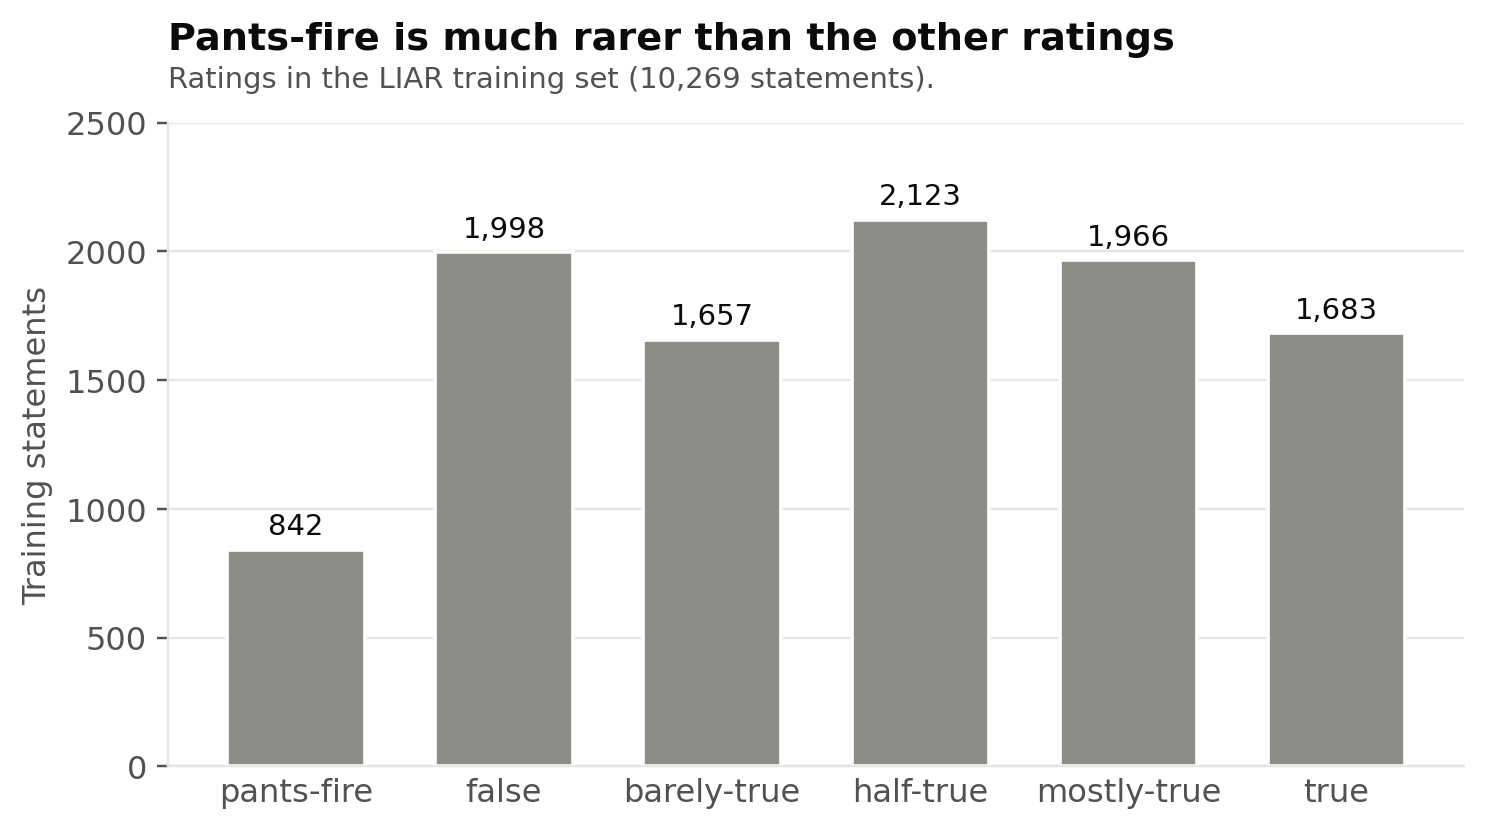
\includegraphics[width=0.78\linewidth]{fig_label_distribution.png}
\caption{Number of training statements per rating.}
\label{fig:dist}
\end{figure}

\subsection{What each statement comes with}
\begin{table}[H]
\centering\small
\caption{Fields available for each statement.}
\begin{tabularx}{\linewidth}{lX}
\toprule
\textbf{Field} & \textbf{What it holds} \\
\midrule
statement & The claim itself, about 18 words on average (longest: 66 words) \\
label & The PolitiFact rating, one of the six levels \\
speaker, job title, state & Who said it, their job and the US state \\
party affiliation & For example republican (4,510 training rows), democrat (3,345), none (1,746) \\
subject & The topic, such as economy (896), health care (745) or education (546) \\
credit history & Five counts of the speaker's past statements rated barely-true, false, half-true, mostly-true and pants-on-fire \\
context & Where the claim was made (a speech, an interview, a post) \\
\bottomrule
\end{tabularx}
\end{table}

The training set has 2,916 different speakers. Many speakers appear many times, which is one reason that
knowing the speaker helps a model.

\subsection{A property of the data that matters later}
In the LIAR release, the five credit-history counts include the rating of the current statement itself. A model
can therefore see part of the answer in the speaker's history. We come back to this in Section~\ref{sec:leak}.

\subsection{Scope}
All statements are short, English, and political, and nearly all are from the United States. The models in this
report know nothing else, and we make no claim about other kinds of news.

% =====================================================================
%  4. METHODOLOGY
% =====================================================================
\section{Methodology}

\subsection{Overview}
Figure~\ref{fig:pipeline} shows how the pieces fit together. A statement goes in, one of three kinds of model
reads it, and a shared scoring step produces the numbers we compare.

\begin{figure}[H]
\centering
\begin{tikzpicture}[
  node distance=7mm and 9mm,
  box/.style={rectangle, rounded corners=3pt, draw=none, fill=softgray, text=ink, align=center,
              minimum height=10mm, minimum width=30mm, font=\sffamily\small},
  inp/.style={box, fill=brandblue!12},
  mdl/.style={box, text=white, minimum width=40mm},
  out/.style={box, fill=brandblue!12},
  arr/.style={-{Stealth[length=2.2mm]}, thick, color=midgray}]
  \node[inp] (in) {Statement\\{\footnotesize + speaker, party,\\ subject, history}};
  \node[mdl, fill=midgray!85, right=of in, yshift=15mm] (lstm) {BiLSTM\\{\footnotesize trained from scratch}};
  \node[mdl, fill=brandblue, right=of in] (bert) {BERT / RoBERTa\\{\footnotesize fine-tuned on LIAR}};
  \node[mdl, fill=brandaqua, right=of in, yshift=-15mm] (llm) {Qwen2.5-7B LLM\\{\footnotesize prompted, no training}};
  \node[out, right=of bert] (score) {Shared scoring\\{\footnotesize accuracy, macro-F1,\\cost, significance test}};
  \draw[arr] (in.east) -- ++(4mm,0) |- (lstm.west);
  \draw[arr] (in.east) -- (bert.west);
  \draw[arr] (in.east) -- ++(4mm,0) |- (llm.west);
  \draw[arr] (lstm.east) -- ++(4mm,0) |- (score.west);
  \draw[arr] (bert.east) -- (score.west);
  \draw[arr] (llm.east) -- ++(4mm,0) |- (score.west);
\end{tikzpicture}
\caption{The pipeline. Three kinds of model, one shared way of scoring them.}
\label{fig:pipeline}
\end{figure}

\subsection{Keeping the comparison fair}
A comparison is only useful if every model is tested in the same way. We therefore fixed the following for all
models.
\begin{itemize}
  \item \textbf{Labels:} the same six labels in the same order.
  \item \textbf{Random seed:} 42 everywhere.
  \item \textbf{Test subset:} the same 300 test statements for every model, chosen so that the mix of ratings matches
        the full test set (22 pants-fire, 59 false, 50 barely-true, 62 half-true, 58 mostly-true, 49 true).
        We use this subset for the headline numbers because the 7B LLM is too slow to run on all 1,283 statements.
        Where we have them, full-test numbers are reported too.
  \item \textbf{Scoring code:} one shared function computes accuracy, macro-F1 and the confusion matrix.
  \item \textbf{Cost:} every model is priced as if it ran on a Tesla T4 GPU at \$0.35 per hour plus 10\% overhead,
        one statement at a time (batch size 1).
\end{itemize}

\textbf{Reference points.} Random guessing scores 16.7\% on six levels. Always answering the most common rating in the
subset (half-true) scores 20.7\%. For the fake-vs-real view in Section~\ref{sec:results}, always guessing the more
common side scores 56.3\%. With only 300 statements, each accuracy is uncertain by about $\pm5$ points.

\subsection{Model 1: BiLSTM baseline}
The LSTM is the simplest model and starts with no knowledge of language. It reads the statement in both directions,
combines the final state with the strongest signal from any word, and outputs six scores.

\begin{itemize}
  \item Word vectors of size 100, learned from scratch; vocabulary of at most 20,000 words seen at least twice in
        the training set only (so nothing leaks from the test set).
  \item One bidirectional LSTM layer with 128 units per direction and dropout 0.5; statements cut at 64 words.
  \item Adam optimiser, learning rate $10^{-3}$, batch size 64, up to 15 epochs with early stopping after 3 epochs
        without improvement; best epoch was the 6th.
  \item Class weights in the loss, so rare ratings count more.
  \item 932,998 trainable parameters. It trains on a CPU in about 4 minutes.
\end{itemize}

\subsection{Models 2 to 5: BERT and RoBERTa}
We fine-tuned \code{bert-base-uncased} (109.5M parameters) and \code{roberta-base} (124.7M parameters) with a new
six-way output layer. Each was trained twice:

\begin{itemize}
  \item \textbf{Text only:} the input is just the statement (up to 128 tokens).
  \item \textbf{With speaker information:} the speaker, party, subject and credit history are written in front of
        the statement (up to 256 tokens).
\end{itemize}

\begin{tcolorbox}[enhanced, colback=softgray, colframe=softgray, arc=2pt, left=8pt, right=8pt, top=5pt, bottom=5pt, fontupper=\small\ttfamily]
speaker: dwayne-bohac | party: republican | subject: abortion | history: 0,1,0,0,0 [SEP] Says the Annies List political group supports third-trimester abortions on demand.
\end{tcolorbox}
\captionof{figure}{Example of the input text for the ``with speaker information'' models (a real training row).}

The training setup was identical for all four runs: AdamW optimiser \cite{loshchilov2019adamw} with learning rate
$2\times10^{-5}$ and weight decay 0.01, batch size 16, 3 epochs, a 10\% warm-up followed by a linear decrease of
the learning rate, gradient clipping at 1.0, mixed-precision (fp16) arithmetic, and inverse-frequency class
weights in the loss. The best epoch was chosen by macro-F1 on the validation set, and it was the last epoch in
every run. We used the Hugging Face Transformers library \cite{wolf2020transformers} on a Colab Tesla T4.

\subsection{Models 6 and 7: the prompted LLM}
We used \code{Qwen2.5-7B-Instruct} \cite{qwen2024} without any training, in 4-bit form (FP4 from the
bitsandbytes library \cite{dettmers2023qlora}) on a Kaggle Tesla T4.

\begin{itemize}
  \item \textbf{Zero-shot prompt:} a system message tells the model it is a fact-checking expert, lists the six labels
        and says ``Respond with ONLY the label, nothing else.'' The statement follows.
  \item \textbf{Few-shot prompt:} the same prompt, plus six worked examples (one per rating) taken from the
        \emph{training} set with seed 42, each 60 to 200 characters long and shuffled so that the last example does not
        favour one rating. Because they come from the training set, none can appear in the test subset.
  \item \textbf{Decoding:} greedy (always the most likely next word), at most 12 new tokens, so runs are repeatable.
  \item \textbf{Strict parsing:} an answer counts only if it contains exactly one valid label. ``Pants on fire'' is
        accepted as pants-fire, but answers with a negation (``not true'') or with two labels are rejected.
        A rejected answer is marked \emph{invalid} and counted as wrong. Parsing therefore never raises the score.
  \item \textbf{No prompt tuning:} each prompt was written once and run once. A 20-statement test checked only that
        the output could be parsed.
  \item \textbf{Input:} the statement only. The LLM was not shown the speaker or party.
\end{itemize}

\subsection{Metrics and statistical test}
\textbf{Accuracy} is the share of statements given exactly the right rating. \textbf{Macro-F1} averages the F1 score
of each of the six ratings, so a model cannot score well by favouring a few common ratings. For the
\textbf{fake-vs-real view} we group pants-fire, false and barely-true as \emph{false-ish} and the other three as
\emph{true-ish}. This grouping is our own choice and was not part of training.

To tell real differences from luck we use \textbf{McNemar's exact test} \cite{mcnemar1947}. It looks only at the
statements where two models disagree, and asks whether one wins more often than chance would allow.

% =====================================================================
%  5. RESULTS
% =====================================================================
\section{Experiments and results}
\label{sec:results}

\subsection{Main results}
Table~\ref{tab:main} gives every score on the shared 300-statement subset. Figure~\ref{fig:acc6} shows the exact-rating
accuracy and Figure~\ref{fig:acc2} the fake-vs-real view.

\begin{table}[H]
\centering\small
\caption{Main results on the shared 300-statement test subset. The two-way column is our own grouping of the saved
predictions. The BiLSTM was timed on a CPU.}
\label{tab:main}
\rowcolors{2}{softgray}{white}
\begin{tabular}{lcccc}
\toprule
\textbf{Model} & \textbf{Accuracy} & \textbf{Macro-F1} & \textbf{Fake vs real} & \textbf{Invalid answers} \\
\midrule
RoBERTa + speaker info & \textbf{0.473} & \textbf{0.483} & \textbf{75.7\%} & 0 / 300 \\
BERT + speaker info    & 0.457 & 0.470 & 75.3\% & 0 / 300 \\
BERT, text only        & 0.293 & 0.289 & 64.0\% & 0 / 300 \\
RoBERTa, text only     & 0.283 & 0.282 & 63.0\% & 0 / 300 \\
Qwen 7B few-shot       & 0.250 & 0.183 & 59.0\% & 0 / 300 \\
BiLSTM                 & 0.190 & 0.173 & 56.3\% & 0 / 300 \\
Qwen 7B zero-shot      & 0.167 & 0.126 & 56.7\% & 1 / 300 \\
\midrule
\multicolumn{5}{l}{\footnotesize Random guessing: 16.7\% (six levels). Always guessing one side: 56.3\% (fake vs real).} \\
\bottomrule
\end{tabular}
\end{table}

\begin{figure}[H]
\centering
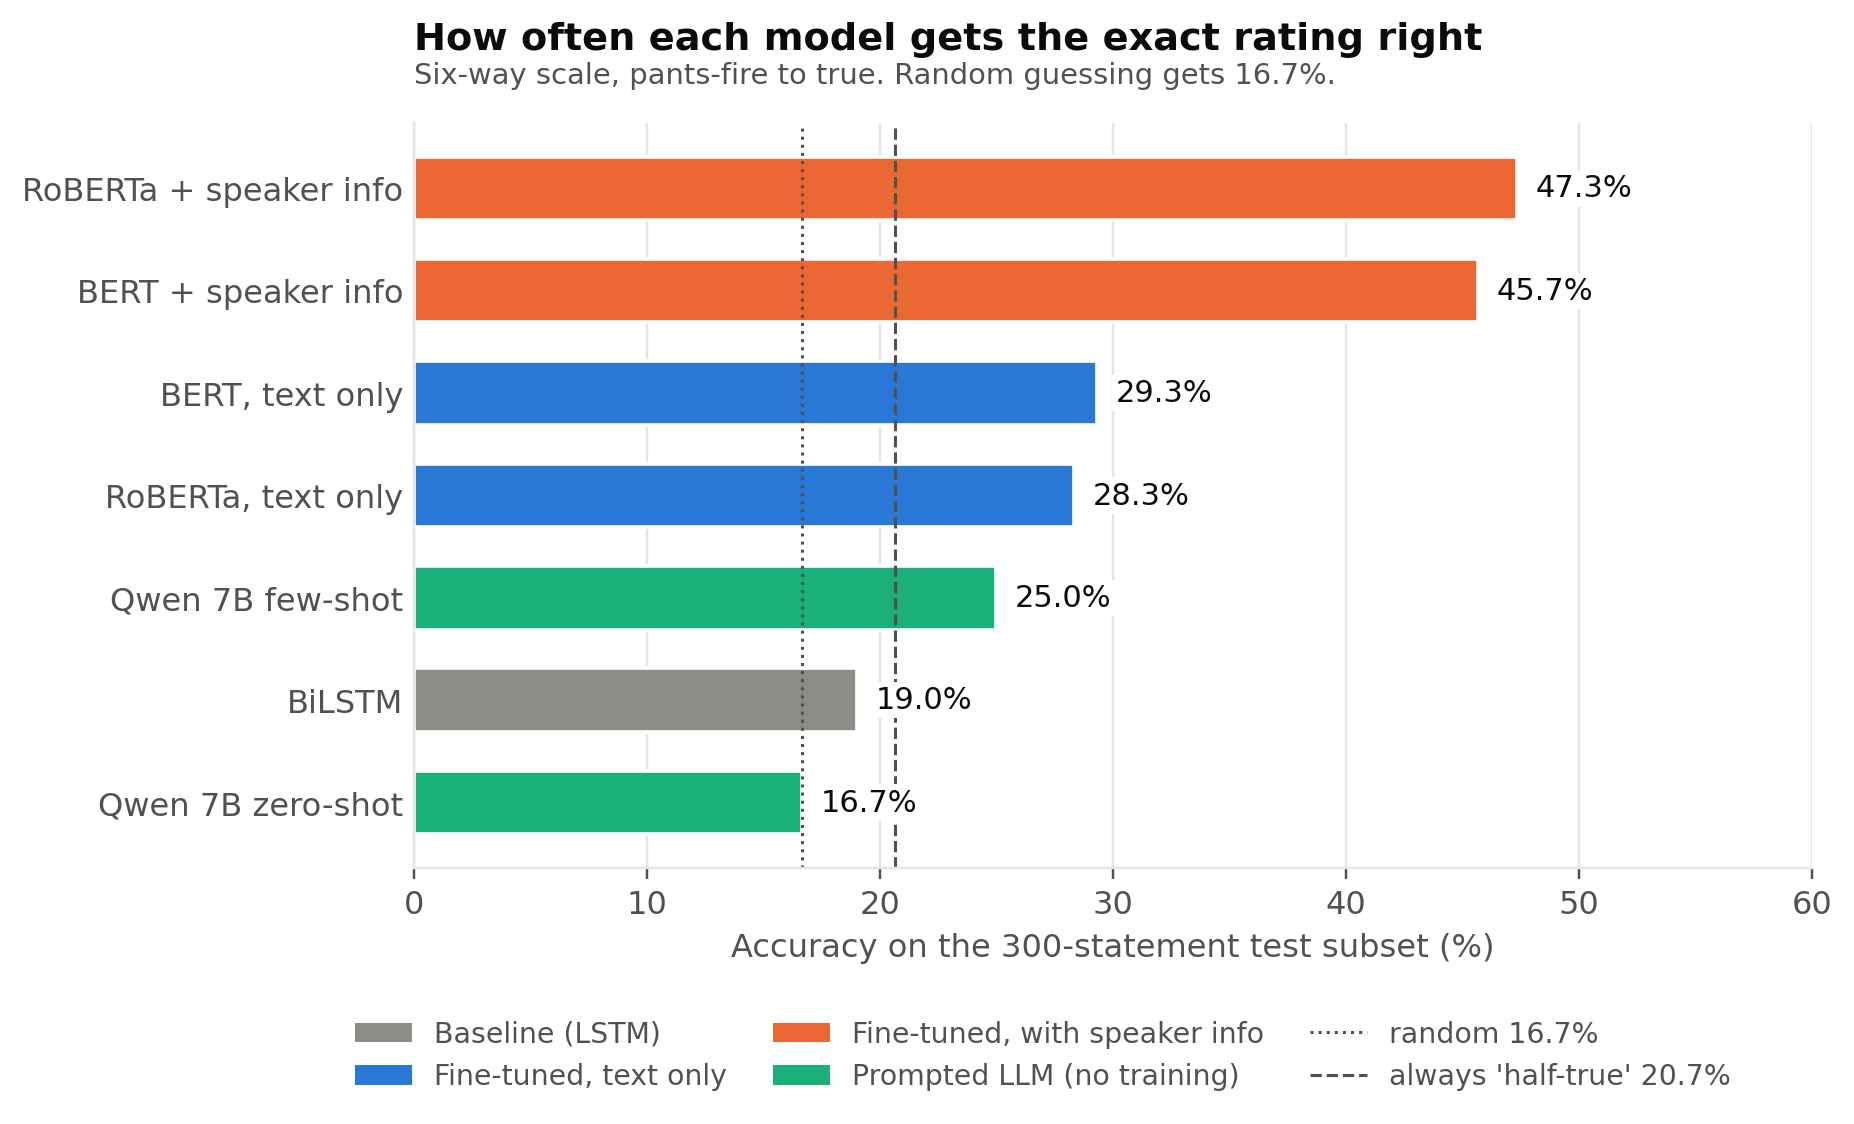
\includegraphics[width=0.92\linewidth]{fig_accuracy_6way.png}
\caption{Exact-rating accuracy on the six-level scale. Colours show the kind of model.}
\label{fig:acc6}
\end{figure}

\begin{figure}[H]
\centering
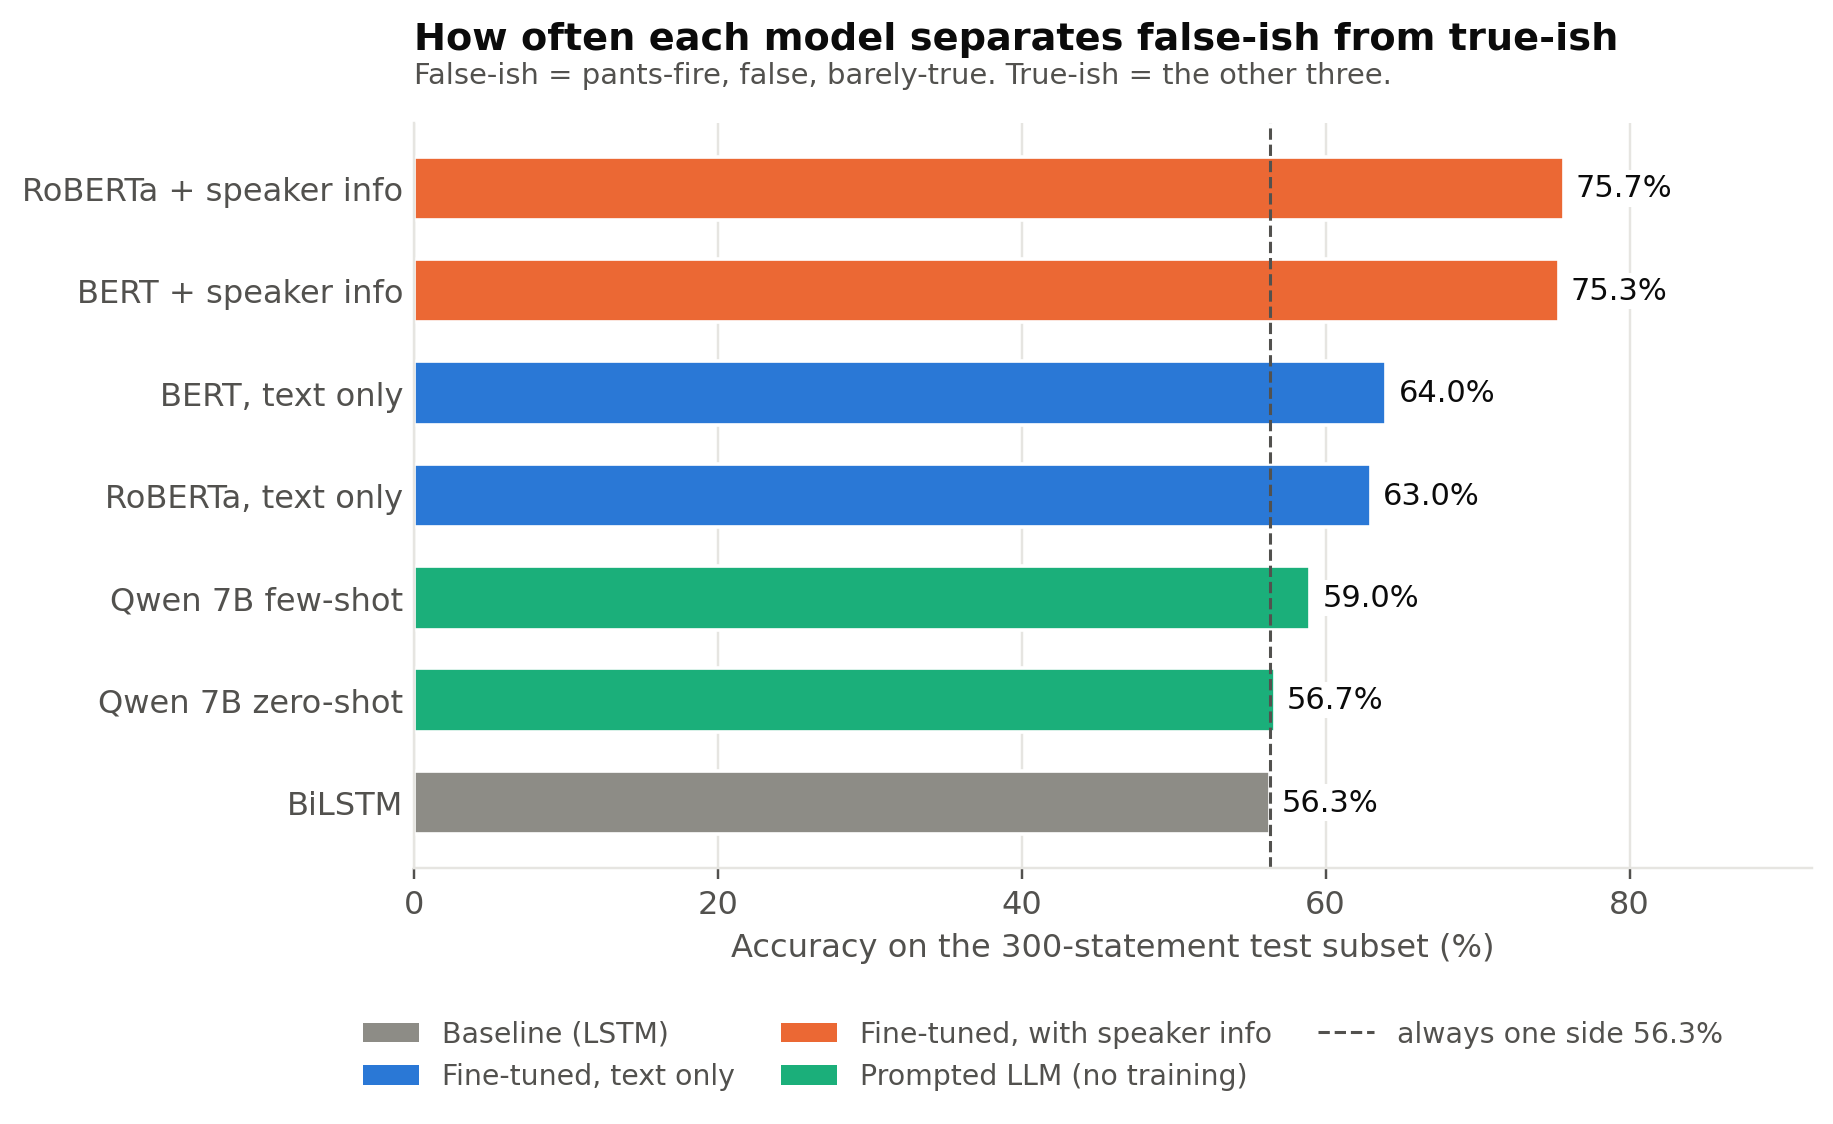
\includegraphics[width=0.92\linewidth]{fig_accuracy_2way.png}
\caption{Accuracy when the six ratings are grouped into false-ish and true-ish.}
\label{fig:acc2}
\end{figure}

\subsection{Results on the full test set}
The 300-statement subset is small, so we also scored the fine-tuned models and the BiLSTM on all 1,283 test statements.
The numbers agree closely with the subset, which gives us more confidence in them. We could not run the LLM on the full set
because it is too slow.

\begin{table}[H]
\centering\small
\caption{Full test set (1,283 statements).}
\rowcolors{2}{softgray}{white}
\begin{tabular}{lcc}
\toprule
\textbf{Model} & \textbf{Accuracy} & \textbf{Macro-F1} \\
\midrule
RoBERTa + speaker info & 0.461 & 0.467 \\
BERT + speaker info    & 0.449 & 0.457 \\
RoBERTa, text only     & 0.288 & 0.291 \\
BERT, text only        & 0.273 & 0.277 \\
BiLSTM                 & 0.212 & 0.201 \\
\bottomrule
\end{tabular}
\end{table}

\subsection{Which ratings are found, and which are missed}
Figure~\ref{fig:recall} shows, for RoBERTa, how many statements of each real rating the model got right.
Speaker information raises the score for five of the six ratings. The exception is \emph{true}, where it falls from
47\% to 29\%. Without speaker information the model finds only 10\% of the half-true statements, the hardest rating for every model.

\begin{figure}[H]
\centering
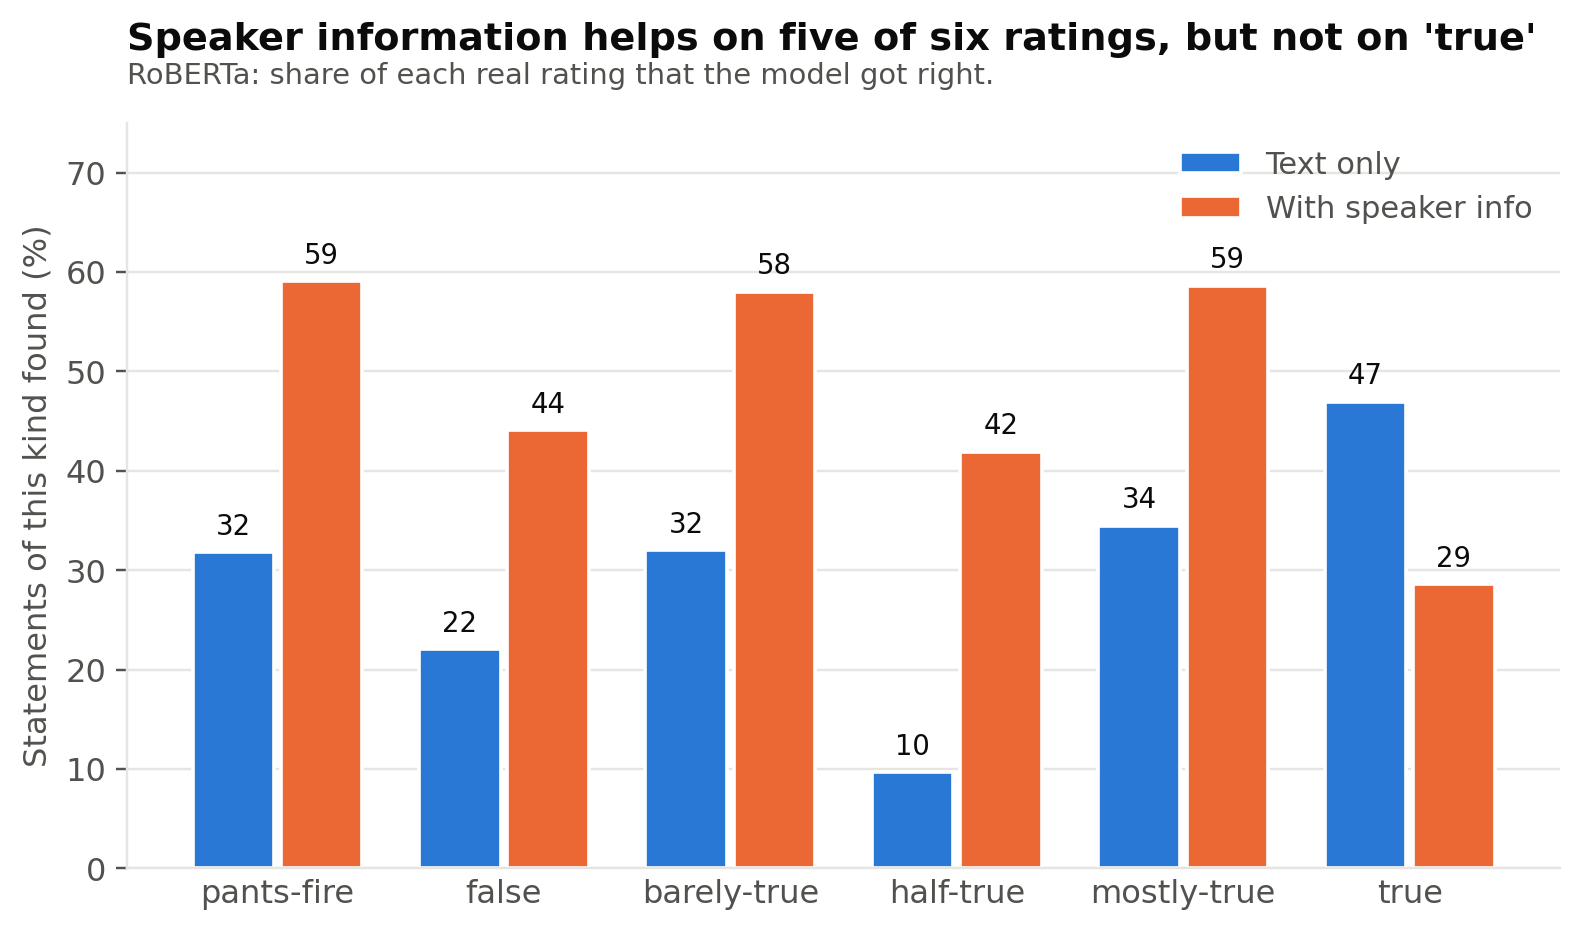
\includegraphics[width=0.85\linewidth]{fig_recall_by_class.png}
\caption{Share of each real rating found by RoBERTa, with and without speaker information (300 statements).}
\label{fig:recall}
\end{figure}

Figure~\ref{fig:conf} shows where the mistakes go. Most wrong answers land on a neighbouring level: for example
\emph{mostly-true} called \emph{true}. Between 42\% and 54\% of all errors are of this near-miss kind.

\begin{figure}[H]
\centering
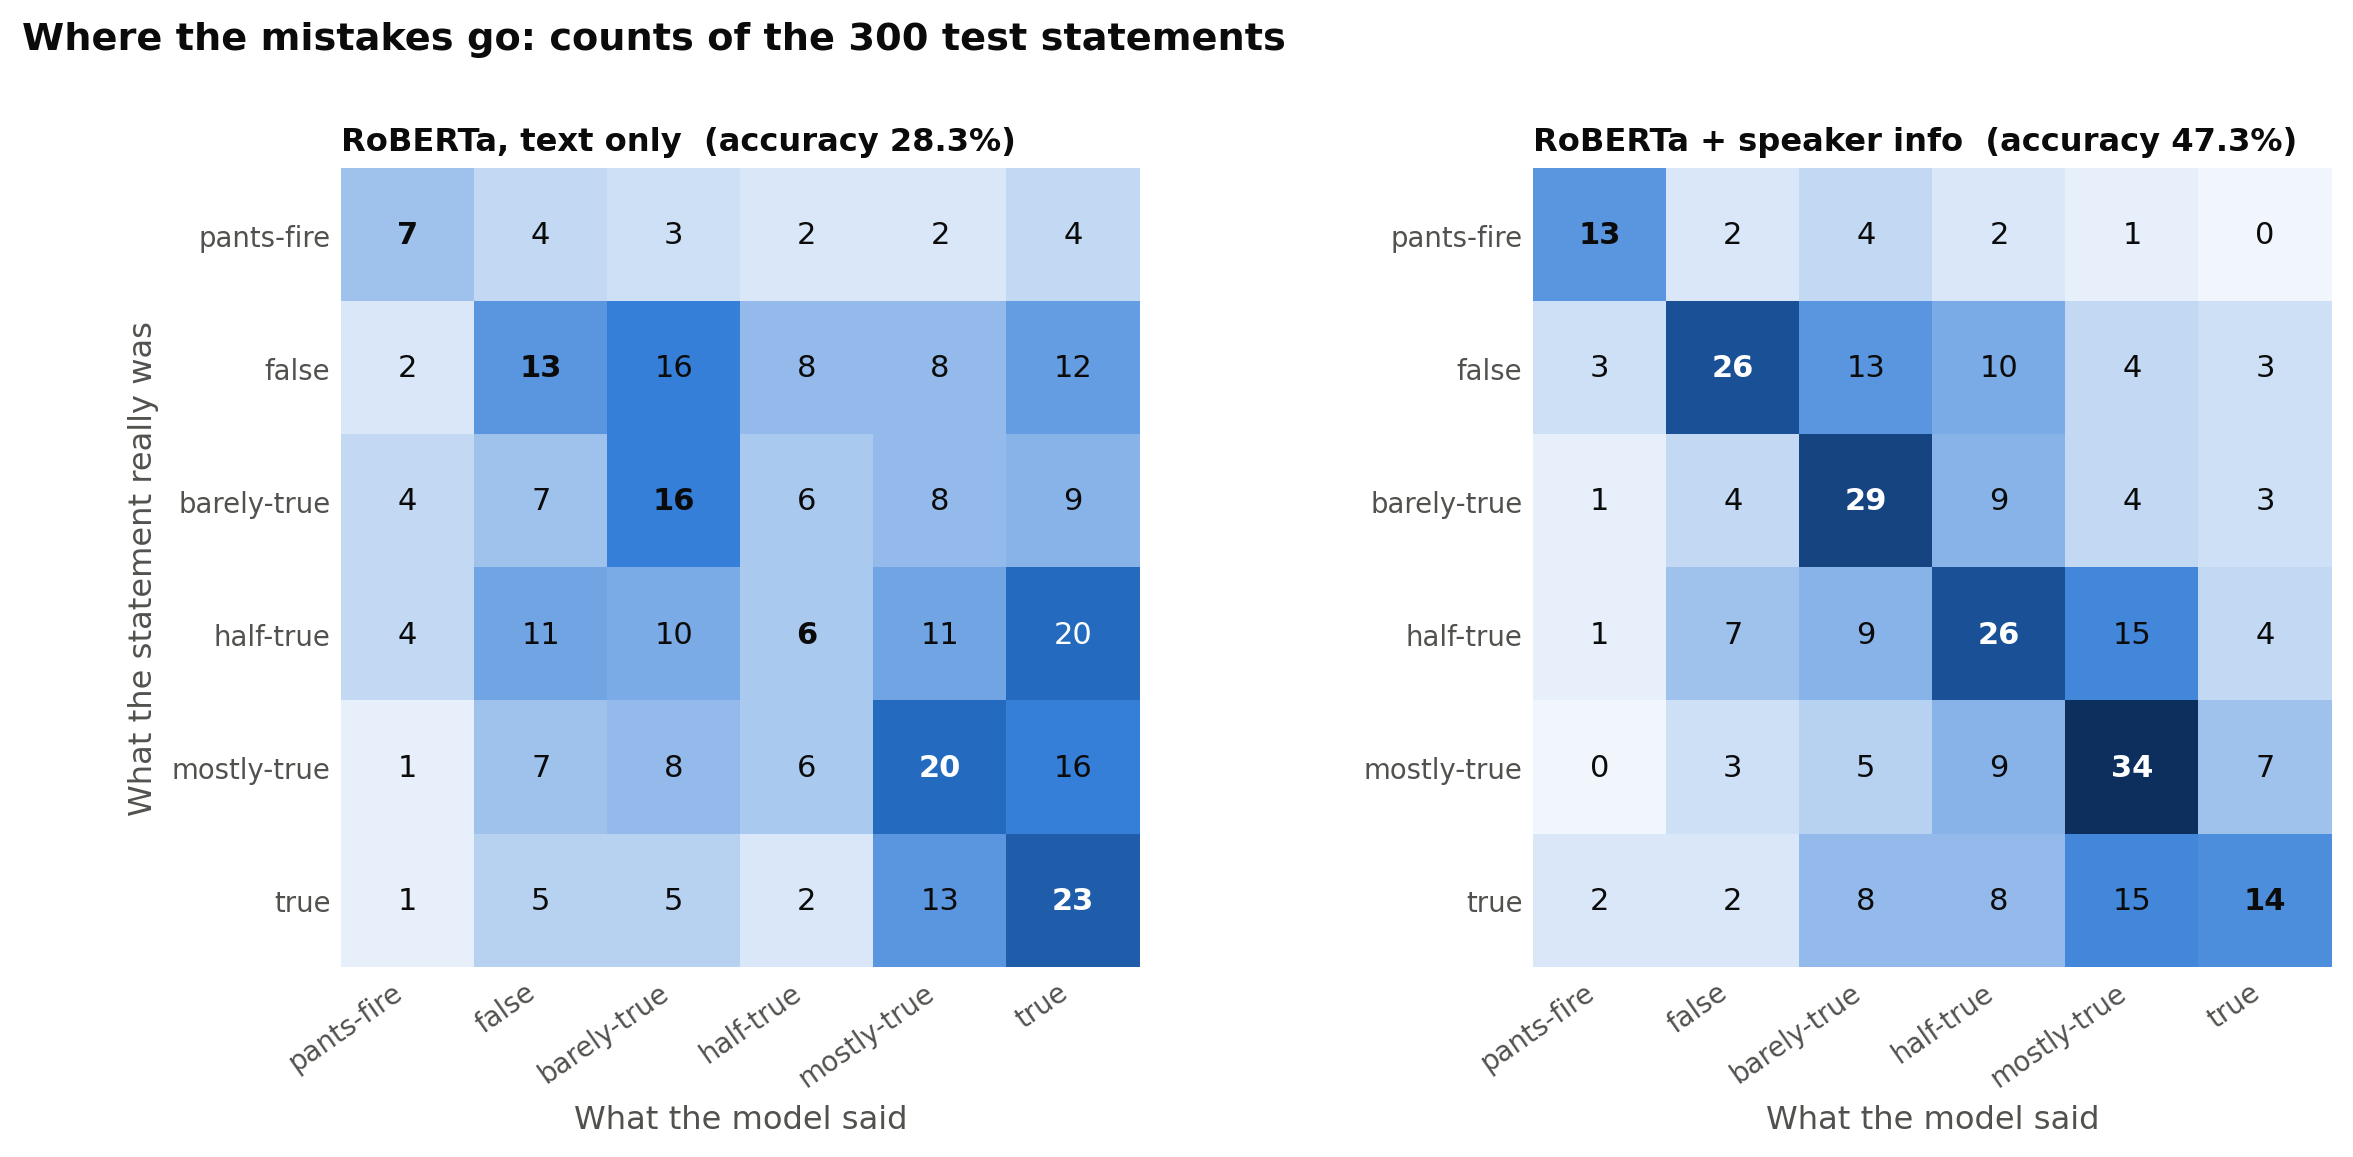
\includegraphics[width=\linewidth]{fig_confusion.png}
\caption{Confusion matrices for RoBERTa. Rows are the real rating, columns are the model's answer.}
\label{fig:conf}
\end{figure}

Two real mistakes from the text-only RoBERTa show how hard the middle ratings are:

\begin{table}[H]
\centering\small
\caption{Two statements rated half-true that the text-only RoBERTa called true.}
\begin{tabularx}{\linewidth}{lX}
\toprule
\textbf{Speaker} & \textbf{Statement} \\
\midrule
facebook-posts & ``1 percent of Americans are millionaires. 47 percent of House Reps. are millionaires. 56 percent of Senators are millionaires.'' \\
nikki-haley & ``Says President Obama and his National Labor Relations Board sued Boeing over its decision to open a plant in South Carolina.'' \\
\bottomrule
\end{tabularx}
\end{table}
Both are true in part and misleading in part, so even a careful human would need the evidence to decide.

\subsection{How the LLM goes wrong}
The LLM does not spread its answers over the six ratings (Figure~\ref{fig:bias}). Zero-shot, it answered
\emph{pants-fire} for 136 of the 300 statements (45\%), although only 22 really are pants-fire, and it almost never
said \emph{true} or \emph{barely-true}. Few-shot moved the bias: it answered \emph{false} for 146 statements (49\%) and
never answered \emph{mostly-true}. Six examples helped, but they did not remove the bias.

\begin{figure}[H]
\centering
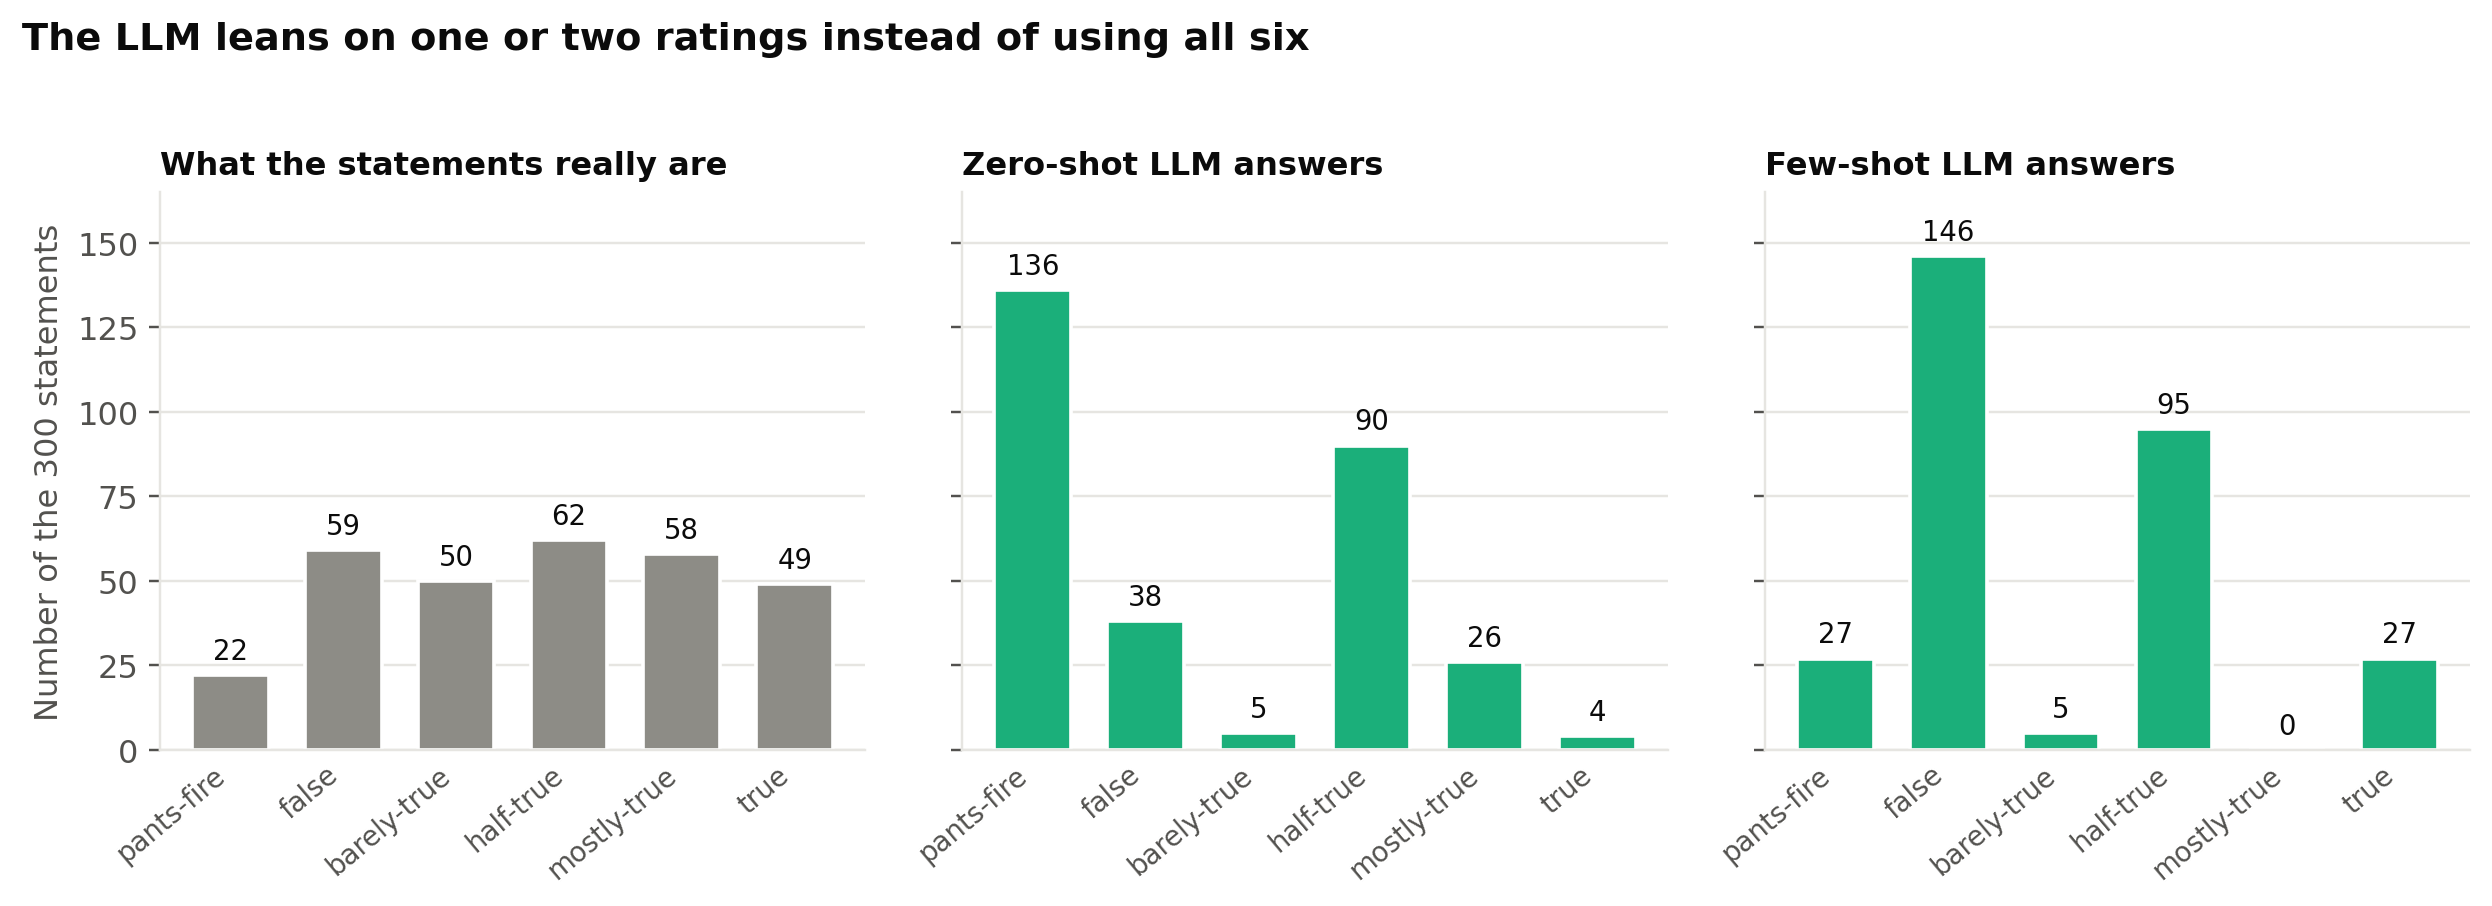
\includegraphics[width=\linewidth]{fig_llm_bias.png}
\caption{What the 300 statements really are (left) and what the LLM answered, zero-shot (middle) and few-shot (right).}
\label{fig:bias}
\end{figure}

\subsection{Are the differences real?}
Table~\ref{tab:sig} lists McNemar tests on the 300 statements.

\begin{table}[H]
\centering\small
\caption{McNemar exact tests. ``Only A right'' counts statements that A got right and B got wrong.}
\label{tab:sig}
\rowcolors{2}{softgray}{white}
\begin{tabular}{llccc}
\toprule
\textbf{Model A} & \textbf{Model B} & \textbf{Only A right} & \textbf{Only B right} & \textbf{p-value} \\
\midrule
Qwen few-shot & Qwen zero-shot & 48 & 23 & 0.004 \\
BERT text only & Qwen few-shot & 66 & 53 & 0.27 \\
BERT text only & Qwen zero-shot & 75 & 37 & 0.0004 \\
BERT + speaker info & BERT text only & 83 & 34 & $<$0.0001 \\
RoBERTa text only & BERT text only & 30 & 33 & 0.80 \\
RoBERTa + speaker info & BERT + speaker info & 30 & 25 & 0.59 \\
\bottomrule
\end{tabular}
\end{table}

How to read it:
\begin{itemize}
  \item \textbf{Few-shot beats zero-shot} ($p=0.004$): the six examples helped, and this is unlikely to be luck.
  \item \textbf{Zero-shot is clearly worse than BERT} ($p=0.0004$) and sits at chance level.
  \item \textbf{BERT vs few-shot in accuracy is not significant} ($p=0.27$). The 4-point gap is within the noise of 300 statements.
        The difference shows up in macro-F1 (0.289 against 0.183), because the LLM favours a few ratings.
  \item \textbf{Speaker information gives a big, real gain} ($p<0.0001$).
  \item \textbf{BERT and RoBERTa are tied.} Their differences are about one point and well inside the noise, so we do not claim one is better.
\end{itemize}

\subsection{Cost and speed}
\label{sec:cost}
Table~\ref{tab:cost} compares size, training time, speed and cost. Figure~\ref{fig:cost} plots cost against accuracy.

\begin{table}[H]
\centering\small
\caption{Size, time and cost, priced at a T4 GPU rate of \$0.35 per hour plus 10\% overhead, batch size 1.}
\label{tab:cost}
\rowcolors{2}{softgray}{white}
\begin{tabular}{lrrrrr}
\toprule
\textbf{Model} & \textbf{Params} & \textbf{Train (min)} & \textbf{Sec / 1,000} & \textbf{\$ / 1,000} & \textbf{GPU (MB)} \\
\midrule
BiLSTM (CPU) & 1M & 3.9 & 2.1 & 0.0002 & n/a \\
BERT, text only & 109M & 3.2 & 14.7 & 0.0016 & 2,144 \\
BERT + speaker info & 109M & 3.8 & 13.9 & 0.0015 & 2,301 \\
RoBERTa, text only & 125M & 3.4 & 14.4 & 0.0015 & 2,429 \\
RoBERTa + speaker info & 125M & 3.9 & 17.3 & 0.0018 & 2,502 \\
Qwen 7B zero-shot & 7,616M & none & 393.5 & 0.0421 & 5,743 \\
Qwen 7B few-shot & 7,616M & none & 661.3 & 0.0707 & 5,789 \\
\bottomrule
\end{tabular}
\end{table}

\begin{figure}[H]
\centering
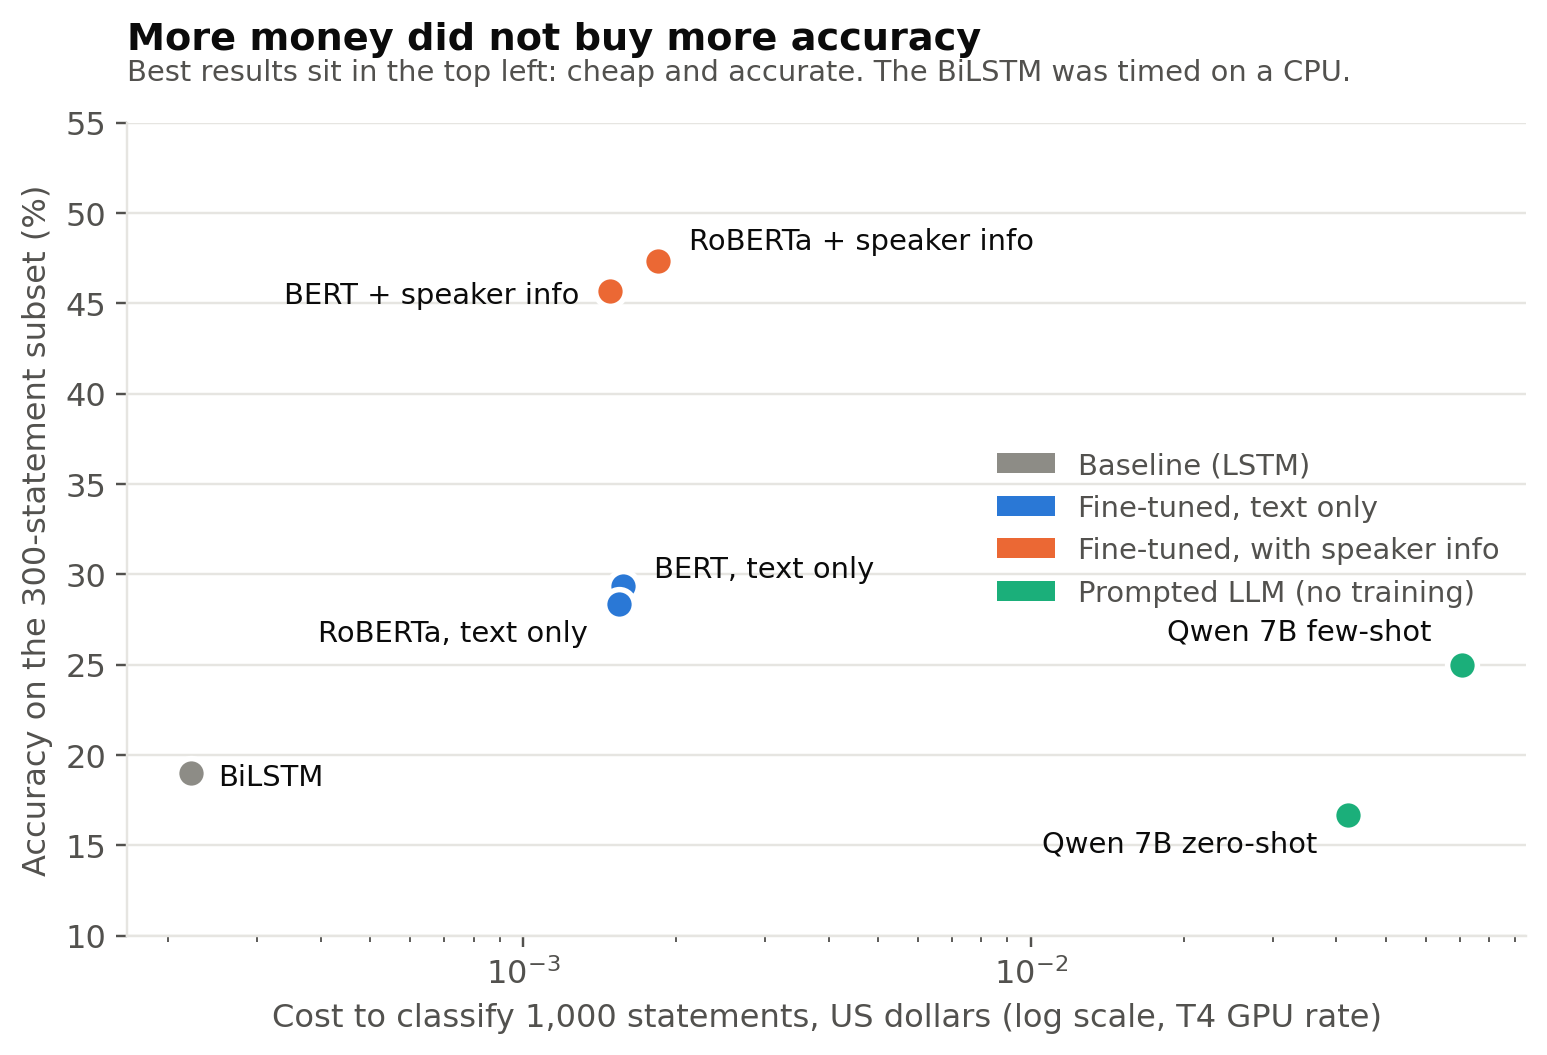
\includegraphics[width=0.88\linewidth]{fig_cost_accuracy.png}
\caption{Cost against accuracy. The best models are in the top left: cheap and accurate.}
\label{fig:cost}
\end{figure}

Compared with the better LLM run (few-shot), text-only BERT is about 70 times smaller, about 45 times faster and
about 45 times cheaper per prediction, and it scores 0.106 higher in macro-F1. BERT's one-off training cost of about
\$0.02 is paid back after roughly 300 predictions. These ratios are an upper bound: we ran the LLM one statement at a time,
and a batching server such as vLLM would narrow the gap.

% =====================================================================
%  6. DISCUSSION
% =====================================================================
\section{Analysis and discussion}

\subsection{What worked}
\begin{itemize}
  \item \textbf{Pre-training matters.} The BiLSTM, which starts from nothing, scored 19\% and is barely above guessing the common
        class. BERT and RoBERTa, which already know English, scored 28--29\% from the same statements.
  \item \textbf{Fine-tuning beats prompting here.} A few minutes of training on 10,000 labelled statements
        taught the small model the six-level scale better than instructions and six examples taught the large one.
  \item \textbf{Knowing the speaker helps a lot.} It was the largest single effect we measured, and it cost only about
        30 seconds more training time.
  \item \textbf{BERT and RoBERTa behave the same.} The choice between them does not matter much for this task.
\end{itemize}

\subsection{Why the LLM struggled}
The six levels are subtle. The gap between barely-true, half-true and mostly-true depends on small details and on
evidence the model does not have. An instruction-following model with no task data seems to turn ``sounds dubious''
into \emph{false} or \emph{pants-fire}, and has no sense of where the middle ratings begin. A fine-tuned model learns
those boundaries from thousands of examples. We tried one model, one prompt and 4-bit weights, so a different
setup might do better, but we did not test it.

\subsection{An important caveat about the best result}
\label{sec:leak}
\begin{warnbox}
The five credit-history numbers are the speaker's record of past ratings, and in the LIAR release they \textbf{already
include the rating of the current statement}. A model can therefore partly read the answer from the speaker's history.
This means the 47\% result is best described as \emph{the value of knowing who is speaking}, not as a better
understanding of the claim.
\end{warnbox}

That is why the fair comparison with the LLM, which sees only the statement, is the \textbf{text-only} models. On a brand-new
statement, where no such history exists, we should expect results closer to the text-only numbers. The cleaner test, using speaker, party and
subject \emph{without} the history counts, has not been run, and it is the first thing we would add.

\subsection{What this means for detecting fake news}
\begin{itemize}
  \item \textbf{As a first-pass signal, it is useful.} On fake vs real, the best model is right about three times out of four,
        against a baseline of 56\%, and the text-only models reach about 64\%.
  \item \textbf{As an automatic judge, it is not good enough.} The best text-only model gets the exact rating right
        fewer than three times in ten. A person should read anything that matters.
  \item \textbf{Near misses are mild.} Many errors move a claim by one level, which is much less harmful than calling
        a false claim true.
\end{itemize}

\subsection{Suggested way to use it}
The following is a suggestion for the team to confirm, not a final decision.
\begin{itemize}
  \item If the speaker is known, use RoBERTa or BERT with speaker information, and check the caveat above before quoting its accuracy.
  \item If only the text is known, use text-only BERT. It matches or beats the prompted 7B LLM at about one forty-fifth of the cost.
  \item We do not recommend the prompted 7B LLM for this task as we set it up: it is slower, costlier and no better.
\end{itemize}

\subsection{Bugs we found and fixed}
\label{sec:bugs}
Running the code on the real dataset, and reviewing each other's pull requests, caught several problems that reading the code did not.
\begin{itemize}
  \item \textbf{Label order mismatch.} The Hugging Face copy of LIAR numbers its labels in a different order from ours.
        The loader crashed, and without a fix every confusion matrix would have been scrambled. Labels are now mapped by name.
  \item \textbf{Credit history lost.} The metadata text looked for a field that does not exist, so every row said
        ``history: 0,0,0,0,0''. It now reads the real count columns.
  \item \textbf{Test subset was not matched to the real mix.} It had 50 statements per rating. It is now proportional,
        and the LSTM was re-run on the corrected subset.
  \item \textbf{Quantization label.} The LLM runs used 4-bit FP4, the library default, and not NF4 as first written. The documentation now says FP4.
\end{itemize}

% =====================================================================
%  7. LIMITATIONS AND ETHICS
% =====================================================================
\section{Limitations and ethics}

\subsection{Limitations}
\begin{itemize}
  \item \textbf{Scope.} The data is short, English, US political statements. We expect worse results on other topics, other
        countries, other languages and full articles, but we did not test them.
  \item \textbf{Small test set.} Three hundred statements means about $\pm5$ points on any accuracy. The LLM was scored only on this subset.
  \item \textbf{One run per setting.} We used a single random seed, so we have not measured run-to-run variation.
  \item \textbf{History counts include the answer.} See Section~\ref{sec:leak}.
  \item \textbf{One LLM, one prompt, 4-bit weights.} Other models (for example Mistral-7B), other prompts, retrieved examples or
        fine-tuning the LLM (QLoRA) could close some of the gap. The LLM also never saw the speaker, so it did not get the same
        information as the speaker-aware models.
  \item \textbf{More epochs might help.} The last epoch was the best for BERT and RoBERTa, so a longer run may add a little.
  \item \textbf{Modest absolute accuracy.} This is normal for LIAR, where text-only models usually score about 25--30\% on six levels.
  \item \textbf{No demo application yet.} We planned a web demo (a FastAPI service and a simple front end), but it was not completed.
\end{itemize}

\subsection{Ethical considerations}
\begin{itemize}
  \item \textbf{The labels are human opinions.} PolitiFact ratings involve judgement. The model learns those judgements, including
        any bias in them.
  \item \textbf{Speaker information can create unfair results.} A model that uses who spoke can learn that some people or parties are
        ``usually false''. That may be statistically true in the data and still be unfair to a particular claim. The speaker-aware
        models should not be used to rate individual people's statements automatically.
  \item \textbf{Mistakes can hurt people.} Calling a true statement false, or the reverse, can damage a reputation or spread a wrong belief.
        We recommend using the model only to help a human reviewer prioritise, with a human making the final call.
  \item \textbf{Do not overstate the numbers.} Our best six-level accuracy is under 50\%. Quote the fake-vs-real figure only with its
        grouping and the leakage caveat.
  \item \textbf{Data and software.} LIAR is a public dataset. We used no private or personal data, no secrets are stored in the code, and all packages are standard, widely used libraries.
        Packages should be checked against your organisation's approved-software list before installation.
\end{itemize}

% =====================================================================
%  8. CONCLUSION
% =====================================================================
\section{Conclusion and future work}

We built and compared seven models for rating the truthfulness of political statements. A small, fine-tuned model was as accurate
as a prompted 7B LLM and clearly better in macro-F1, while being about 70 times smaller and 45 times cheaper. Adding the speaker
raised accuracy from about 29\% to about 46\%, giving a best result of 47.3\% on six levels and 75.7\% on fake vs real.
Statement text alone gives 28--29\% on six levels, which is typical for this hard dataset.

The main lesson is that, for a narrow task with labelled data, training a small model is better than prompting a large one,
both in quality and in cost. The model is a helper for human reviewers, not a replacement for them.

\textbf{Future work.}
\begin{enumerate}
  \item Run the missing test with speaker, party and subject but \emph{without} the history counts.
  \item Build the demo application (service and web page) so the model can be tried on any statement.
  \item Train on more varied data, such as other fake-news datasets, to widen the scope beyond US politics.
  \item Repeat each run with several seeds and score the LLM on more statements.
  \item Try other LLMs and prompts, retrieved examples, and fine-tuning the LLM with QLoRA.
  \item Measure speaker bias directly, for example by comparing results across parties.
\end{enumerate}

% =====================================================================
%  REFERENCES
% =====================================================================
\begin{thebibliography}{99}
\addcontentsline{toc}{section}{References}

\bibitem{wang2017liar} W.~Y. Wang. ``Liar, Liar Pants on Fire'': A New Benchmark Dataset for Fake News Detection.
\emph{Proceedings of ACL (Short Papers)}, 2017, pp.~422--426. arXiv:1705.00648.

\bibitem{devlin2019bert} J.~Devlin, M.-W. Chang, K.~Lee, K.~Toutanova. BERT: Pre-training of Deep Bidirectional
Transformers for Language Understanding. \emph{Proceedings of NAACL}, 2019, pp.~4171--4186. arXiv:1810.04805.

\bibitem{liu2019roberta} Y.~Liu et al. RoBERTa: A Robustly Optimized BERT Pretraining Approach. 2019. arXiv:1907.11692.

\bibitem{hochreiter1997lstm} S.~Hochreiter, J.~Schmidhuber. Long Short-Term Memory. \emph{Neural Computation}, 9(8):1735--1780, 1997.

\bibitem{vaswani2017attention} A.~Vaswani et al. Attention Is All You Need. \emph{Advances in Neural Information
Processing Systems}, 2017. arXiv:1706.03762.

\bibitem{brown2020fewshot} T.~Brown et al. Language Models are Few-Shot Learners. \emph{Advances in Neural Information
Processing Systems}, 2020. arXiv:2005.14165.

\bibitem{qwen2024} Qwen Team. Qwen2.5 Technical Report. 2024. arXiv:2412.15115.

\bibitem{dettmers2023qlora} T.~Dettmers, A.~Pagnoni, A.~Holtzman, L.~Zettlemoyer. QLoRA: Efficient Finetuning of
Quantized LLMs. \emph{Advances in Neural Information Processing Systems}, 2023. arXiv:2305.14314.

\bibitem{loshchilov2019adamw} I.~Loshchilov, F.~Hutter. Decoupled Weight Decay Regularization. \emph{ICLR}, 2019. arXiv:1711.05101.

\bibitem{wolf2020transformers} T.~Wolf et al. Transformers: State-of-the-Art Natural Language Processing.
\emph{Proceedings of EMNLP: System Demonstrations}, 2020, pp.~38--45.

\bibitem{mcnemar1947} Q.~McNemar. Note on the sampling error of the difference between correlated proportions or percentages.
\emph{Psychometrika}, 12(2):153--157, 1947.

\end{thebibliography}

% =====================================================================
%  APPENDICES
% =====================================================================
\appendix
\section{Training settings}
\label{app:settings}

\begin{table}[H]
\centering\small
\caption{Settings for every trained model.}
\rowcolors{2}{softgray}{white}
\begin{tabular}{lccc}
\toprule
\textbf{Setting} & \textbf{BiLSTM} & \textbf{BERT / RoBERTa} & \textbf{Qwen 7B} \\
\midrule
Training data & train split & train split & none \\
Optimiser & Adam & AdamW & not trained \\
Learning rate & $10^{-3}$ & $2\times10^{-5}$ & -- \\
Batch size & 64 & 16 & 1 (inference) \\
Epochs (max) & 15 & 3 & -- \\
Early stopping & 3 epochs & 2 epochs & -- \\
Best epoch & 6 & 3 & -- \\
Max length & 64 words & 128 / 256 tokens & 12 new tokens \\
Class weights & yes & yes & -- \\
Seed & 42 & 42 & 42 (few-shot picks) \\
Hardware & CPU & Colab T4 & Kaggle T4 \\
Precision & fp32 & fp16 & 4-bit FP4 \\
\bottomrule
\end{tabular}
\end{table}

\section{The LLM prompt}
The system message used for both LLM runs:
\begin{quote}\small\itshape
You are a fact-checking expert. Classify the given political statement by its truthfulness using exactly one of these labels:
pants-fire (ridiculously false), false, barely-true, half-true, mostly-true, true. Respond with ONLY the label, nothing else.
\end{quote}
Each statement is then given as ``Statement: \ldots{} Label:''. The few-shot run places six worked examples as earlier
question-and-answer turns in the same format.

\section{How the work was organised}
We tracked the work as GitHub issues (data, evaluation, each model, analysis and documentation), each done on its own branch
and merged through a pull request. Teammates reviewed each other's pull requests, and several of the bugs in
Section~\ref{sec:bugs} were found that way. The shared pieces (labels, data loader, scoring code, test subset) were built first so the
model work could run in parallel.

\section{How to reproduce the results}
\label{app:repro}
\begin{enumerate}
  \item Install the packages in \code{requirements.txt} (check them against your approved-software list first).
  \item Run the tests: \code{python -m pytest tests/ -q}. All 99 should pass.
  \item Train the BiLSTM: \code{python -m baselines.train} (a CPU is enough).
  \item Train BERT and RoBERTa and run the LLM on a GPU (a Colab or Kaggle T4 is enough). The steps are in
        \code{colab/RUN\_COLAB.md} and \code{llm/RUN\_COLAB.md}.
  \item Results are written to \code{results/}. The full cost table is \code{results/cost\_comparison.md}.
  \item Rebuild the figures in this report with \code{python report/make\_figures.py}.
\end{enumerate}

\end{document}
